\documentclass[11pt,a4paper]{article}
\usepackage{jheppub}
\usepackage{amssymb}
\usepackage{amsmath}
\usepackage{graphicx}
\usepackage{tikz}
\newcommand{\expval}[1]{\left\langle#1\right\rangle}
\newcommand{\dd}{\mathrm{d}}
\renewcommand{\vec}[1]{\boldsymbol{#1}}

\title{One-loop PDF of the average Ising magnetization in 4 dimensions.}
\author[a]{Andrea Allais}
\affiliation[a]{Independent scholar}
\emailAdd{allais.andrea@gmail.com}
\abstract{We compute at one loop in perturbation theory the probability density
function of the average magnetization $\bar{\phi}$ of the Ising model on both
the 4-torus and the 4-sphere. The perturbative expansion covers the entire
symmetric phase and a neighborhood of the critical point. We find that, at the
critical point, the PDF has the asymptotic behavior $p(\bar{\phi})\sim
\exp(-f(R) \bar{\phi}^4)$, and hence the critical value of the Binder cumulant
is $U = 1 - \frac{4\,\Gamma(5/4)^2}{ 3\,\Gamma(3/4)^2}$. We validate our
results by comparison with Monte Carlo simulation.}
\begin{document}

\maketitle

\section{Main results}

The average magnetization $\bar{\phi} = \frac{1}{V} \sum_{i} \sigma_i$ of the
Ising model is the simplest observable in Monte Carlo simulations. For large
system size, the probability distribution of $\bar{\phi}$ changes qualitatively
between the two phases of the model. In the symmetric phase, if the correlation
length $\xi$ is large in lattice units, but small compared to the system size
$L$, the distribution is well approximated by a normal distribution centered at
0. In the broken symmetry phase, still for $1 \ll \xi \ll L$, the distribution
is well approximated by a bimodal superposition of two normals centered at
non-zero values $\pm \bar{\phi}_0$. 

Near the critical point $1 \ll L \ll \xi$ the probability distribution of
$\bar{\phi}$ is a non-trivial function of $\bar{\phi}$, at least in two and
three dimensions.  It is not immediately clear if the same is true in four
dimensions as well.  Since the $\phi^4$ field theory that describes the Ising
critical point in four dimensions becomes weakly coupled in the infrared, one
may expect the probability distribution to be a single zero-centered normal at
the critical point as well.

To clarify this issue, we compute the log pdf of $\bar{\phi}$ at one-loop in
$4$ dimensions, and show that for very large system size, the critical
probability distribution is not normal, but rather of the form
$-\log p(\bar{\phi})\sim f(L) \bar{\phi}^4$. We find that corrections to this
form vanish very slowly with increasing system size, like $1/\log L$.

\begin{figure}
\begin{center}
\includegraphics[scale=0.75]{binder_cumulant.png}
\end{center}
    \caption{\label{fig:binder_cumulant} Binder cumulant of the total
    magnetization of the 4D Ising model. The left plot gives a broad picture,
    the right plot shows the critical region close-up.  The shaded regions
    display the one-sigma confidence intervals obtained from Monte Carlo
    simulation. The center lines are obtained from a 3-parameter fit of the
    perturbative result (\ref{eq:log_pdf}). The horizontal dashed line
    indicates the critical value (\ref{eq:critical_binder_cumulant}). The fit
    has $J_c = 0.1496938$, $J - J_c = -0.027\cdot r$, $g = 0.43$, with $r$, $g$
    defined at the renormalization scale $L = 2\pi R = 8$. }
\end{figure}


Thus we consider the $\phi^4$ field theory with action:
\begin{equation}
  S[\phi] \equiv \int \dd^4 x\ \left(
    \frac{1}{2} \phi\left(\Delta + r_0\right)\phi +
    \frac{1}{24} u_0 \phi^4\right)
\end{equation}
defined on a 4-torus of radius $R$, i.e. $x_i\sim x_i + 2\pi R$. In this field
theory context, the pdf of the average magnetization is defined as:
\begin{equation}
    \label{eq:pdf_definition}
    p(\bar\phi) \equiv \frac{1}{Z} \int \left[\mathcal{D}\phi\right]
    \delta\left(\bar{\phi} - \frac{1}{V}\int\dd^4 x\ \phi\right)
    e^{-S[\phi]}\,,
\end{equation}
and at one loop it evaluates to:
\begin{equation}
\label{eq:log_pdf}
\begin{split}
    -\log p(\bar{\phi}) = \mathrm{const.} +  V\Bigg(
  &\frac{1}{2} \frac{\bar{\phi}^2}{R^2} \left(
    r R^2 + \frac{g}{6} \left(f_1\left(r R^2\right) - 1\right)
    + O\left(g^2\right)\right) + \\
  & \frac{2\pi^2}{9}g\bar{\phi}^4\left(
    1 - \frac{g}{2}f_2\left(r R^2\right)
    + O\left(g^2\right)\right) + \\
  & \frac{8\pi^4}{81} g^3 \bar{\phi}^6 R^2\left(
    f_3\left(r R^2\right)
    + O\left(g\right)\right) + O\left(g^4\bar{\phi}^8\right) \Bigg)\,,
\end{split}
\end{equation}
where the coefficients $r$ and $g$ are the renormalized counterparts to $r_0$
and $u_0$. An explicit expression for the functions $f_1$, $f_2$ and $f_3$ is
reported in the appendix (\ref{eq:f_functions}), and they are plotted in
fig.~\ref{fig:f_functions}.

\begin{figure}
\begin{center}
\includegraphics[scale=0.75]{f_functions.png}
\end{center}
\caption{\label{fig:f_functions} The functions $f_i$ that appear in
    (\ref{eq:log_pdf}). The functions go to zero as $x\to\infty$, and diverge
    for $x\to-1$ ($x\to-4$ for the sphere), signaling an instability of the
    perturbative vacuum.}
\end{figure}

Eq. (\ref{eq:log_pdf}) is our central result, and we now describe it
at lenght. We first illustrate its domain of validity and its dependence on the
renormalized couplings $r$, $g$ on a torus of fixed radius $R$, then describe
its dependence on $R$ at fixed bare couplings $r_0$, $u_0$.

The dimension-2 coupling $r$ controls the cross-over between the symmetric and
broken-symmetry phases. The expression (\ref{eq:log_pdf}) is valid for
all positive values of $r$, and also for negative values, provided that $rR^2
\gtrsim -1/2$.  For lower values of $r$, additional modes of the laplacian
condense beside the zero-mode, and this invalidates the perturbative expansion.
. This becomes manifest in a divergence of the functions $f_i$ as their
argument approaches -1.  On the other hand, $f_1$, $f_2$, $f_3$ all go to zero
as their argument approaches positive infinity, and hence for large $r$ the
probability distribution of $\bar{\phi}$ is a zero-centered normal:
\begin{equation}
    p(\bar{\phi}) \sim N e^{- \frac{1}{2} V r \bar{\phi}^2}
  \quad \text{for} \quad
  rR^2 \gg 1\,.
\end{equation}

The dimensionless coupling $g$ is the parameter of the perturbative expansion.
The expansion is valid for $g \ll 1$, provided $rR^2$ is sufficiently far from
the bound discussed above.

In order to describe how $p(\bar{\phi})$ depends on $R$ at fixed bare couplings
$r_0$, $u_0$, it is necessary to account for renormalization effects. In
general, the renormalized couplings $r$, $g$ depend on a renormalization scale
$\mu$, and it is possible to derive an expression for $p(\bar{\phi})$ evaluated
at a generic value of $\mu$. However, for simplicity,
(\ref{eq:log_pdf}) is evaluated at the scale $\mu^2 = r + R^{-2}$.
This choice of $\mu$ is optimal for the reliability of perturbation theory,
because it avoids the emergence of large logarithms over the widest possible
range of parameters.

The renormalization group equations for $r$ and $g$ are:
\begin{equation}
  \label{eq:renormalization_group}
  \mu \frac{\dd g}{\dd \mu} = g^2\,,\quad
  \mu \frac{\dd r}{\dd \mu} = \frac{1}{3}g r\,.
\end{equation}

These can be integrated and combined with the condition $\mu^2 = r + R^{-2}$ to
obtain a system of equations\footnote{There are of course many alternative,
arguably simpler, solutions that differ by subleading orders in an expansion in
$g(R_1)$. The one displayed here is the exact solution to
(\ref{eq:renormalization_group}).} connecting the renormalized couplings at two
different values of $R$:
\begin{equation}
  \frac{g(R_1)}{g(R_2)} = \frac{r(R_1)^3}{r(R_2)^3} = 
  1 - \frac{1}{2} g(R_1)\log\frac{r(R_2) + R_2^{-2}}{r(R_1) + R_1^{-2}}\,.
\end{equation}

\begin{figure}
\begin{center}
\includegraphics[scale=0.75]{renormalization_group.png}
\end{center}
    \caption{\label{fig:renormalization_group} A few solutions to
    (\ref{eq:renormalization_group}) with $g(R_1) = 0.45$.  In the left plot,
    the shaded region shows where the perturbative expansion becomes invalid.
    Similarly in the right plot, the lines become dotted oustside of the
    perturbative region. Note how the sign of $r$ is preserved, $r = 0$ is a
    solution, and $g$ goes to $0$ for $R_2 \gg R_1$.}
\end{figure}

A few solutions to these equations are shown in
fig.~\ref{fig:renormalization_group}. Within the perturbative regime $g \ll 1$,
$r R^2 \gtrsim -1/2$, the coupling $r$ varies very little with $R$, and, as is
clear from the differential form (\ref{eq:renormalization_group}), the sign of
$r$ is always preserved. Thus we conclude that the critical point is at $r
= 0$, and the symmetric phase is realized for $r > 0$.

At the critical point, the renormalized coupling $g$ follows the simplified renormalization group equation:
\begin{equation}
    \frac{1}{g(R_2)} - \frac{1}{g(R_1)} = \log\frac{R_2}{R_1}\,,
\end{equation}
and hence, as system size grows, the renormalized coupling $g$ goes to zero.
In this regime, the quartic term in (\ref{eq:log_pdf}) dominates all the
others. This is perhaps most evident if the PDF is expressed in terms of the
rescaled quantity $\bar{\varphi} = g^{\frac{1}{4}} \bar{\phi}$, whose
variance remains finite as $g\to0$.

Thus we conclude that, for sufficiently large system size: 
\begin{equation}
    \label{eq:log_pdf_critical_point}
    -\log p(\phi) \sim \mathrm{const} + \frac{2\pi^2}{9} V g\bar{\phi}^4\,,
\end{equation}
with subleading terms vanishing like $1 / \log(R)$.

In Monte Carlo simulations, the qualitative behavior of the distribution of the
magnetization is often characterized by measuring the so-called Binder
cumulant \cite{Binder1981}:
\begin{equation}
    U = 1 - \frac{\left\langle \bar \phi^4 \right \rangle}
    {3\left\langle \bar \phi^2 \right \rangle^2},
\end{equation}
which is constructed to be independent of the overall scale of $\bar{\phi}$,
and to be zero if $\bar{\phi}$ is normally distributed. From
(\ref{eq:log_pdf_critical_point}) we conclude that, on a 4-Torus, at the
critical point\footnote{ Incidentally, we note that this result is not in
contraddiction with the claim in the original paper \cite{Binder1981} that the
critical Binder cumulant in 4 dimensions is zero, because in the original paper
the cumulant is not computed from the total magnetization, but rather from the
average magnetization of blocks of spins much smaller than the overall system
size.}:
\begin{equation}
    \label{eq:critical_binder_cumulant}
    U = 1 - \frac{4\,\Gamma\left(\frac{5}{4}\right)^2}
    {3\,\Gamma\left(\frac{3}{4}\right)^2} 
    = 0.27052\ldots
\end{equation}


In fig.~\ref{fig:binder_cumulant}, we show a comparison of the Binder cumulant
computed from (\ref{eq:log_pdf}) near the critical point, and the results of
Monte Carlo simulation of the $4D$ Ising model. The agreement is excellent except
for the smallest system size $L = 8$, probably because of contributions from
irrelevant operators. Notice how slowly the finite size Binder cumulant
approaches the asymptotic value (\ref{eq:critical_binder_cumulant}).

\section{Derivation on the 4-torus}

We now describe briefly how the result (\ref{eq:log_pdf}) is obtained. The
perturbative approach is very similar to the computation of the effective
action, as in \textit{e.g.} \cite{WeinbergEffectiveAction}, except that we are
interested in the whole probability distribution of $\bar{\phi}$, instead of
just the expected value. The main difficulty lies in evaluating the loop
integrals at finite size.

First of all we observe that the average magnetization
$\bar{\phi}$ is proportional to the zero momentum mode of the field $\phi$:
\begin{equation}
    \phi(x) = \frac{1}{V} \sum_{n \in \mathbb{Z}^4} \phi_{n} 
    e^{i \frac{n\cdot x}{R}}\,;\quad \bar{\phi} = \frac{\phi_{0}}{V}\,.
\end{equation}

Thus, because of the delta function in (\ref{eq:pdf_definition}), the component
$\phi_{0}$ becomes an external field, whereas the other components $\phi_{n}$
with are still part of the functional integral. Separating the zero momentum
mode from the other modes in the action yields:
\begin{equation}
\begin{split}
    S(\bar{\phi}, \phi) =& 
    V \left(\frac{1}{2} r_0 \bar{\phi}^2 + \frac{u_0}{24} \bar{\phi}^4\right) +
    \frac{u_0}{4V} \bar{\phi}^2 \sum_{n} \phi_{n} \phi_{-n} + \\
    &\frac{u_0}{6V^2} \bar{\phi} 
        \sum_{n_1, n_2} \phi_{n_1} \phi_{n_2} \phi_{-n_1 -n_2} + \\
    &\frac{u_0}{24V^3} \sum_{n_1, n_2, n_3} \phi_{n_1} \phi_{n_2} 
        \phi_{n_3} \phi_{-n_1 -n_2 -n_3}\,,
\end{split}
\end{equation}
where all summations now exclude $n = (0, 0, 0, 0)$.

We also introduce renormalized couplings
\begin{equation}
    u_0 = u(1 + u\delta u)\,;\quad r_0 = r(1 + u \delta r)\,,
\end{equation}
and we obtain the following edges and vertices in the diagrammatic expansion:
\begin{displaymath}
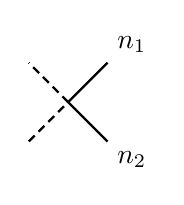
\begin{tikzpicture}[scale=0.5, baseline=(current bounding box.center)]
    \draw[densely dashed, thick] (-1, -1) -- (0, 0) -- (-1, 1);
    \draw[thick] (+1, -1) -- (0, 0) -- (+1, 1);
    \node[above right] at (1, 1) {$n_1$};
    \node[below right] at (1, -1) {$n_2$};
\end{tikzpicture}
    -\frac{u\bar{\phi}^2}{4V}\delta_{n_1 + n_2}
    \quad\quad
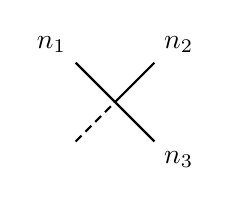
\begin{tikzpicture}[scale=0.5, baseline=(current bounding box.center)]
    \draw[densely dashed, thick] (-1, -1) -- (0, 0);
    \draw[thick] (0, 0) -- (-1, 1);
    \draw[thick] (+1, -1) -- (0, 0) -- (+1, 1);
    \node[above left] at (-1, 1) {$n_1$};
    \node[above right] at (1, 1) {$n_2$};
    \node[below right] at (1, -1) {$n_3$};
\end{tikzpicture}
    -\frac{u\bar{\phi}}{6V^2}\delta_{n_1 + n_2 + n_3}
\end{displaymath}
\begin{displaymath}
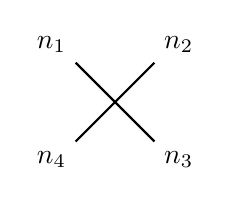
\begin{tikzpicture}[scale=0.5, baseline=(current bounding box.center)]
    \draw[thick] (-1, -1) -- (1, 1);
    \draw[thick] (-1, 1) -- ( 1, -1);
    \node[above left] at (-1, 1) {$n_1$};
    \node[above right] at (1, 1) {$n_2$};
    \node[below right] at (1, -1) {$n_3$};
    \node[below left] at (-1, -1) {$n_4$};
\end{tikzpicture}
    -\frac{u}{24V^3}\delta_{n_1 + n_2 + n_3 + n_4}
\quad\quad
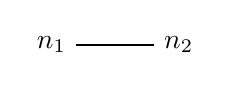
\begin{tikzpicture}[scale=0.5, baseline=(current bounding box.center)]
    \draw[thick] (-1, 0) -- (1, 0);
    \node[left] at (-1, 0) {$n_1$};
    \node[right] at (1, 0) {$n_2$};
\end{tikzpicture}
    \quad
    \frac{V}{n_1^2R^{-2} + r}\delta_{n_1 + n_2}
\end{displaymath}
plus additional vertices associated with the counterterms $\delta r$, $\delta
u$ which we do not list for brevity.

The logarithm of the probability distribution of $\bar{\phi}$ is the sum of all
connected diagrams:
\begin{displaymath}
\begin{split}
    \log p(\bar{\phi}) = &\,
    \mathrm{const} -V \left(\frac{1}{2} r \bar{\phi}^2 + 
    \frac{u}{24} \bar{\phi}^4\right)\\
&+\ 
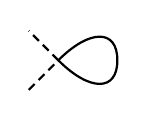
\begin{tikzpicture}[scale=0.5, baseline={([yshift=-.5ex]current bounding box.center)}]
    \draw[thick, densely dashed] (-1.75, -0.75) -- (-1, 0) -- (-1.75, 0.75);
    \draw[thick] (-1, 0) .. controls (-0.2, 0.8) and (0.5, 0.8) .. (0.5, 0) .. 
    controls (0.5, -0.8) and (-0.2, -0.8) .. (-1, 0);
\end{tikzpicture}
\ + \ 
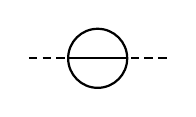
\begin{tikzpicture}[scale=0.5, baseline={([yshift=-.5ex]current bounding box.center)}]
    \draw[thick, densely dashed] (-1.75, 0) -- (-0.75, 0);
    \draw[thick] (-0.75, 0) -- (0.75, 0);
    \draw[thick, densely dashed] (1.75, 0) -- (0.75, 0);
    \draw[thick] (0, 0) circle (0.75cm);
\end{tikzpicture}
\ + \ 
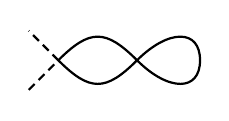
\begin{tikzpicture}[scale=0.5, baseline={([yshift=-.5ex]current bounding box.center)}]
    \draw[thick, densely dashed] (-2.75, -0.75) -- (-2, 0) -- (-2.75, 0.75);
    \draw[thick] (-2, 0) .. controls (-1.2, 0.8) and (-0.8, 0.8) .. (0, 0) .. 
    controls (-0.8, -0.8) and (-1.2, -0.8) .. (-2, 0);
    \draw[thick] (1.6, 0) .. controls (1.6, 0.8) and (0.8, 0.8) .. (0, 0) .. 
    controls (0.8, -0.8) and (1.6, -0.8) .. (1.6, 0);
\end{tikzpicture}
 \ + \ \cdots \\
&+\ 
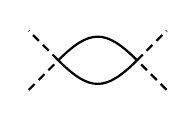
\begin{tikzpicture}[scale=0.5, baseline={([yshift=-.5ex]current bounding box.center)}]
    \draw[thick, densely dashed] (-1.75, -0.75) -- (-1, 0) -- (-1.75, 0.75);
    \draw[thick, densely dashed] (1.75, -0.75) -- (1, 0) -- (1.75, 0.75);
    \draw[thick] (-1, 0) .. controls (-0.2, 0.8) and (0.2, 0.8) .. (1, 0) .. 
    controls (0.2, -0.8) and (-0.2, -0.8) .. (-1, 0);
\end{tikzpicture}
\ + \ 
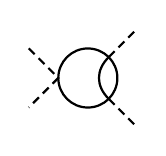
\begin{tikzpicture}[scale=0.5, baseline={([yshift=-.5ex]current bounding box.center)}]
    \draw[thick, densely dashed] (-1.5, 0.75) -- (-0.75, 0) -- (-1.5, -0.75) ;
    \draw[thick] (0, 0) circle (0.75cm);
    \draw[thick, densely dashed] (0.53, 0.53) -- (1.25, 1.25);
    \draw[thick, densely dashed] (0.53, -0.53) -- (1.25, -1.25);
    \draw[thick] (0.53, -0.53) .. controls (0.2, -0.2) 
    and (0.2, 0.2) .. (0.53, 0.53);
\end{tikzpicture}
\ + \ 
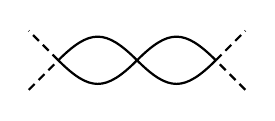
\begin{tikzpicture}[scale=0.5, baseline={([yshift=-.5ex]current bounding box.center)}]
    \draw[thick, densely dashed] (-2.75, -0.75) -- (-2, 0) -- (-2.75, 0.75);
    \draw[thick, densely dashed] (2.75, -0.75) -- (2, 0) -- (2.75, 0.75);
    \draw[thick] (-2, 0) .. controls (-1.2, 0.8) and (-0.8, 0.8) .. (0, 0) .. 
    controls (-0.8, -0.8) and (-1.2, -0.8) .. (-2, 0);
    \draw[thick] (2, 0) .. controls (1.2, 0.8) and (0.8, 0.8) .. (0, 0) .. 
    controls (0.8, -0.8) and (1.2, -0.8) .. (2, 0);
\end{tikzpicture}
 \ + \ \cdots \\
& + \ 
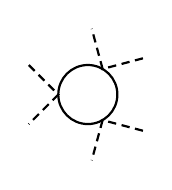
\begin{tikzpicture}[scale=0.5, baseline={([yshift=-.5ex]current bounding box.center)}]
    \draw[thick, densely dashed] (-1.5, 0.75) -- (-0.75, 0) -- (-1.5, -0.75) ;
    \draw[thick] (0, 0) circle (0.75cm);
    \draw[thick, densely dashed] (1.40, -0.92) -- (0.375, -0.65) -- (0.1, -1.67);
    \draw[thick, densely dashed] (1.40, 0.92) -- (0.375, 0.65) -- (0.1, 1.67);
\end{tikzpicture}
 \ + \ \cdots \,,
\end{split}
\end{displaymath}
where again we left out all diagrams involving the counterterms for brevity. 

Retaining only one-loop diagrams, and employing a heath kernel regulator we have:
\begin{equation}
\begin{split}
    -\log p(\bar{\phi}) = \mathrm{const} + V \Bigg( 
    &\frac{1}{2} \bar{\phi}^2\left( r + u \left(\delta r + \frac{1}{2} I_1\right) + O(u^2)\right) + \\
    &\frac{u}{24} \bar{\phi}^4 \left(1 + u \left(\delta u - \frac{3}{2} I_2\right) + O(u^2)\right) + \\
    &\frac{u^3}{48}\bar{\phi}^6\left(I_3 + O(u)\right) + O(u^4 \bar{\phi}^8) \Bigg)\,,
\end{split}
\end{equation}
where
\begin{equation}
    I_k = \frac{1}{V} \sum_{n\in\mathbb{Z}^4\setminus\{0\}} 
    \frac{e^{-s(r + n^2 R^{-2})}}{\left(r + n^2 R^{-2}\right)^k} = 
    \frac{1}{(k - 1)!}\left(-\frac{\partial}{\partial r} - s\right)^k I_1
\end{equation}

The summation $I_1$ can be simplified substantially using the following trick:
\begin{equation}
\begin{split}
    I_1 &= \frac{1}{V} \int_{s}^{\infty} \dd t \sum_{n\in\mathbb{Z}^4\setminus\{0\}} 
    e^{-t(r + n^2 R^{-2})}\\
    & = \frac{1}{V} \int_{s}^{\infty} \dd t\ e^{-t r}
        \left(\left(\sum_{m = -\infty}^{\infty} e^{-t m^2 R^{-2}}\right)^4 - 1\right) \\
    & = \frac{1}{V} \int_{s}^{\infty} \dd t\ e^{-t r}
        \left(\theta\!\left(t R^{-2}\right)^4 - 1\right)\,,
\end{split}
\end{equation}
where:
\begin{equation}
    \label{eq:theta}
    \theta(z) = \theta_3(0, e^{-z}) = \sum_{m = -\infty}^{\infty} e^{-m^2 z}\,.
\end{equation}
Here $\theta_3$ is a Jacobi theta function, but we will not need any of
its special properties beyond its asymptotic behavior, which can be easily
obtained from the definition.

We now extract the divergent and finite parts of $I_1$ as $s\to 0$ by
subtracting under the integral a function that has the same asymptotic behavior
as the integrand for $t \to 0$, but whose integral can be computed in closed
form. In order to do that, we need the asymptotic behavior of $\theta(z)$ for
$z\to0$, which can be obtained from its definition using the Euler-Mclaurin
formula:
\begin{equation}
    \theta(z) \sim \sqrt{\frac{\pi}{z}} + o(z^k) \quad\mathrm{for}\, z\to0\,.
\end{equation}

Thus we have:
\begin{equation}
\begin{split}
    I_1 &= \frac{1}{16\pi^2}\left(\int_{s}^{\infty}\dd t\, e^{-t \mu^2} t^{-2}\left(1 + t (\mu^2 - r)\right)
    +\frac{1}{R^2} f(r R^2, \mu R) + O(s)\right)\\
    &= \frac{1}{16\pi^2}\left(\frac{1}{s} + r\left(\log s\mu^2 + \gamma_{E}\right) - 
    \mu^2 +\frac{1}{R^2} f(r R^2, \mu R) + O(s)\right)\,,
\end{split}
\end{equation}
where $\mu$ is a renormalization scale that can be chosen at will, and:
\begin{equation}
    \label{eq:f_definition}
    f(\bar{r},\bar{\mu}) = \int_{0}^{\infty} \dd z\ e^{-z \bar{r}} \left(\frac{\theta(z)^4 - 1}{\pi^2} - 
    \frac{1 + z\left(\bar{\mu}^2 - \bar{r}\right)}{z^2}e^{-z\left(\bar{\mu}^2 - \bar{r}\right)}\right).
\end{equation}

We set the counterterms to:
\begin{align}
    &\delta r = -\frac{1}{32\pi^2}\left(\frac{1}{s} + r\left(\log s \mu^2 + \gamma_E - 1\right)\right)\,,\\
    &\delta u = -\frac{3}{32\pi^2}\left(\log s\mu^2 +\gamma_E + 1\right)\,,
\end{align}
from which the renormalization group equations (\ref{eq:renormalization_group})
can be obtained, and we have:
\begin{equation}
\begin{split}
    -\log p(\bar{\phi}) =& \mathrm{const}+ V \Bigg( \\
    &\frac{1}{2} \bar{\phi}^2\left( r + \frac{u}{32\pi^2}  \left(\left(\frac{1}{R^2} f(rR^2, \mu R) + r - \mu^2\right)\right) + O(u^2)\right) + \\
    &\frac{u}{24} \bar{\phi}^4 \left(1 + \frac{3u}{32\pi^2} f^{(1, 0)}(rR^2, \mu R) + O(u^2)\right) + \\
    &\frac{u^3}{48}\bar{\phi}^6\left(\frac{R^2}{32\pi^2}f^{(2, 0)}(rR^2, \mu R) + O(u)\right) + O(u^4 \bar{\phi}^8) \Bigg)\,,
\end{split}
\end{equation}
from which (\ref{eq:log_pdf}) is obtained by setting $g = \frac{3 u}{16
\pi^2}$ and $\mu^2 = r + R^{-2}$. This last choice is motivated as follows. The
subtraction in (\ref{eq:f_definition}) is similar to:
\begin{equation}
    \int_0^{\infty} \dd z\, \frac{e^{-a z} - e^{-b z}}{z} = \log \frac{b}{a}\,;
\end{equation}
when the asymptotic behavior of the two terms for large $z$ is not well
matched, the integral becomes large in magnitude, making the perturbative
expansion less reliable. With the choice $\mu^2 = r + R^{-2}$, both terms in
(\ref{eq:f_definition}) have the same asymptotic behavior $\sim e^{-z(\bar{r} +
1)}$, thus avoiding the large log problem over the widest possible range of
parameters.

For completeness, let us display explicitly the functions $f_i$ that
parametrize (\ref{eq:log_pdf}):
\begin{align}
\label{eq:f_functions}
    &f_1(\bar r) = f(\bar r, \sqrt{\bar r + 1}) = 
    \int_{0}^{\infty} \dd z\ e^{-z \bar{r}} \left(\frac{\theta(z)^4 - 1}{\pi^2} - 
    \frac{(1 + z) e^{-z}}{z^2}\right)\,,\\
    &f_2(\bar r) = f^{(1, 0)}(\bar r, \sqrt{\bar r + 1}) = 
    \int_{0}^{\infty} \dd z\ e^{-z \bar{r}} z \left(\frac{\theta(z)^4 - 1}{\pi^2} - 
    \frac{e^{-z}}{z^2}\right)\,,\\
    &f_3(\bar r) = f^{(2, 0)}(\bar r, \sqrt{\bar r + 1}) = 
    \int_{0}^{\infty} \dd z\ e^{-z \bar{r}} z^2 \frac{\theta(z)^4 - 1}{\pi^2}\,,
\end{align}
and $\theta$ is given by (\ref{eq:theta}).

\section{Results for the 4-sphere}
\label{sec:four_sphere}
It is possible to obtain $\log p(\bar{\phi})$ on the 4 sphere as well, with
very similar methods. Here we highlight the main differences from the 4 torus.

Curved manifolds allow for an additional renormalizable coupling: 
\begin{equation}
    S += \int \dd^4 x\ \frac{1}{2}\xi_0 \phi^2 \mathcal{R}\,,
\end{equation}
where $\mathcal{R}$ is the scalar curvature and $\xi_0$ is a dimensionless bare
coupling. On a static manifold, this coupling is equivalent to a mass term.
The free theory is Weyl invariant if $\xi_0 = \frac{1}{6}$. In the
presence of interactions, the coupling needs to be renormalized as well, and
its renormalized counterpart $\xi$ becomes a running coupling. At one loop, the
renormalization group equation for $\xi$ is:
\begin{equation}
    \mu \frac{\dd \xi}{\dd \mu} =  \frac{1}{3} g \left(\xi - \frac{1}{6}\right)\,.
\end{equation}

From this experssion it seems that $\xi$ can be set to the critical value
$\frac{1}{6}$ at all energy scales. However, this turns out to be an illusion:
at higher orders in perturbation theory the renormalization group equation
becomes inhomogeneous \cite{Brown1980}. Therefore, on a curved manifold, $\xi$
is simply another free parameter of the scalar field theory.

The probability distribution of the total magnetization on the 4-sphere is
still given by (\ref{eq:log_pdf}), with the substitution:
\begin{equation}
    rR^2 \to \frac{\xi}{12} + r R^2\,
\end{equation}
where $R$ is now the radius of the sphere, and with the functions $f_i$ defined
as:
\begin{align}
    &f_1(\bar{r}) = (2 - \bar{r})\int \dd z\ e^{-z(\bar{r} + 4)} \left(H(z) - \frac{1}{z}\right) + \frac{7}{3}\,,\\
    &f_2(\bar{r}) = \int \dd z\ e^{-z(\bar{r} + 4)} 
    \left(1 + z (2 - \bar{r})\right) \left(H(z) - \frac{1}{z}\right)+ \frac{6}{\bar{r} + 4}\,,\\
    &f_3(\bar{r}) = \int \dd z\ e^{-z(\bar{r} + 4)} 
    \left(2 + z (2 - \bar{r})\right)z \left(H(z) - \frac{1}{z}\right) + \frac{\bar{r} + 10 }{(\bar{r} + 4)^2}\,,\\
\end{align}
where:
\begin{equation}
    H(z) = \sum_{\ell = 1}^{\infty} (2\ell + 3)e^{-z (\ell(\ell + 3) - 4)}\,.
\end{equation}

The functions $f_i$ for the sphere are also displayed in
fig.~\ref{fig:f_functions}. They diverge for $\bar{r} \to -4$, signaling the
instability of the perturbative vacuum, and they go to zero for $\bar{r} \to
\infty$.


\begin{thebibliography}{9}
\bibitem{Binder1981}
K. Binder,
\textit{Critical Properties from Monte Carlo Coarse Graining and Renormalization},
\href{https://doi.org/10.1103/PhysRevLett.47.693}{Phys. Rev. Lett. \textbf{47} (1981) 693}.

\bibitem{WeinbergEffectiveAction}
S. Weinberg,
\textit{The quantum theory of fields, Vol. 2}, Cambridge University Press, (1996) pg. 63.

\bibitem{Brown1980}
Lowell S. Brown, John C. Collins,
\textit{Dimensional renormalization of scalar field theory in curved space-time},
\href{https://doi.org/10.1016/0003-4916(80)90232-8}{Ann. Phys. \textbf{130} (1980) 215}.
\end{thebibliography}



\end{document}


The coupling $\eta$ is related to the coupling between the scalar and
the curvature, and hence it is exactly zero on the tourus. On the sphere, it
may seem that it can be set to a constant value $\eta = 2$ at all energy
scales, however this ceases to be true at higher orders in perturbation theory,
where the renormalization group equation becomes inhomogeneous.



